\subsection{NAND}
    The NAND gate, short for NOT-AND, is a versatile logic gate that can be obtained by connecting an AND gate and a NOT gate in series, as shown in Figure \ref{fig:NAND_gate}. \\
    The NAND gate's operation can be algebraically represented as $\text{NAND}(A, B) = \overline{A \cdot B}$, where $A$ and $B$ are the input signals.
    When all inputs are high (1), all the transistors in the AND part conduct, resulting in a high output (1) for the AND operation. 
    The NOT gate then inverts this high output to a low final output (0).
    This behavior is consistent with the NAND gate's truth table shown in Table \ref{tab:NAND_table}. \\
    The symbol for the NAND gate is shown in Figure \ref{fig:NAND_sym}. 

    \begin{figure}[H]   
        \begin{minipage}{0.5\textwidth}
            \centering
            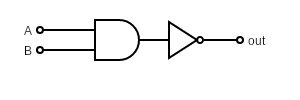
\includegraphics[width=1.1\textwidth]{figures/circuits/NAND.png}
            \captionof{figure}{NAND gate.} 
            \label{fig:NAND_gate} 
        \end{minipage}
        \begin{minipage}{0.5\textwidth}
            \centering
            \captionof{table}{NAND truth table.}
            \begin{tabular}{|c|c|c|}
                \hline
                Input A & Input B & Output \\
                \hline
                0 & 0 & 1 \\
                0 & 1 & 1 \\
                1 & 0 & 1 \\
                1 & 1 & 0 \\
                \hline
            \end{tabular}
            \label{tab:NAND_table}
        \end{minipage}
	\end{figure}

    \begin{figure}[H]
	    \centering
	    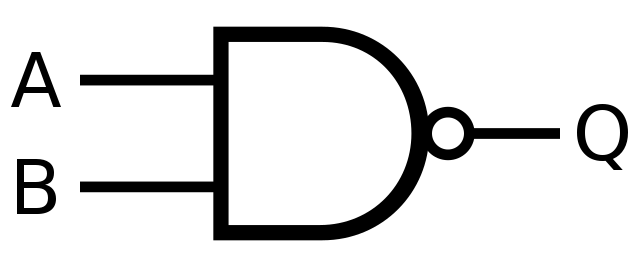
\includegraphics[width=0.3\textwidth]{figures/symbols/NAND.png}
	    \caption{NAND symbol.}
	    \label{fig:NAND_sym} 
	\end{figure}